\newpage
\section{Resoconti di verifica ed esiti delle revisioni}

In questa sezione vengono mostrati i valori delle metriche calcolate a termine del periodo di progettazione architetturale. Saranno mostrati sia i valori che rientrano nel range prestabilito sia quelli che non rientrano, nel secondo caso verranno segnalati come problemi nelle conclusioni che sranno divise per fasi.

\subsection{Valori dell'indice di Gulpease}

Per ogni documento stilato è stato calcolato l'indice di Gulpease\glo{}. I valori sono dati dalla seguente tabella ed il rispettivo grafico con valore sufficiente >40 e valore ottimo >80.

\hphantom{}
\tabulinesep = 2mm % padding
\taburowcolors [1] 2{pari .. dispari} % colori delle righe

\begin{longtabu} to \textwidth {| X[0.2,c m]  | X[0.1,c m] | X[0.1,c m]| X[0.1,c m] | X[0.1,c m] |}
\hline
\rowcolor{header}
\textbf{Data del calcolo} &  
\textbf{Norme di Progetto} & 
\textbf{Analisi dei Requisiti} & 
\textbf{Piano di Qualifica} & 
\textbf{Piano di Progetto} \\
\hline

\multirow[c]{2}{*}{2020-12-03} & v0.1.0 & v0.2.4 & v0.2.1 & v0.1.0 \\
\cline{2-5} 
& 65 & 61 & 80 & 91 \\ 
\hline
\multirow[c]{2}{*}{2021-01-10} & v1.0.0 & v1.0.0 & v1.0.0 & v1.0.0 \\ 
\cline{2-5} 
 & 68 & 69 & 70 & 79 \\ 
\hline
\multirow[c]{2}{*}{2021-02-05}  & v1.0.1 & vx.0.0 & v1.0.2 & v1.0.2 \\ 
\cline{2-5} 
 & x & x & x & x \\ 
\hline
\multirow[c]{2}{*}{2021-02-20}  & v1.1.3 & vx.0.0 & v1.1.2 & v1.0.3 \\ 
\cline{2-5} 
 & x & x & x & x \\ 
\hline
\multirow[c]{2}{*}{2021-03-09} & v2.0.0 & v2.0.0 & v2.0.0 & v2.0.0 \\ 
\cline{2-5} 
 & x & x & x & x \\ 
\hline
\end{longtabu}


\begin{figure}[H]
    \centering
    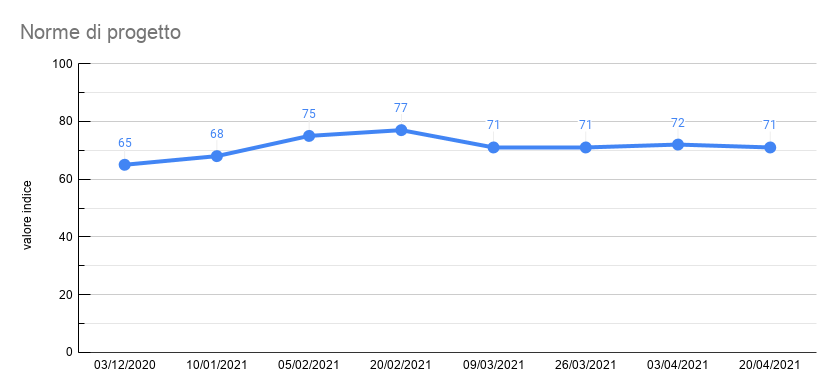
\includegraphics[width=13 cm]{source/sections/images/IdG_NdP.png}
    \caption{Indice di Gulpease - Norme di Progetto}
\end{figure}

\begin{figure}[H]
    \centering
    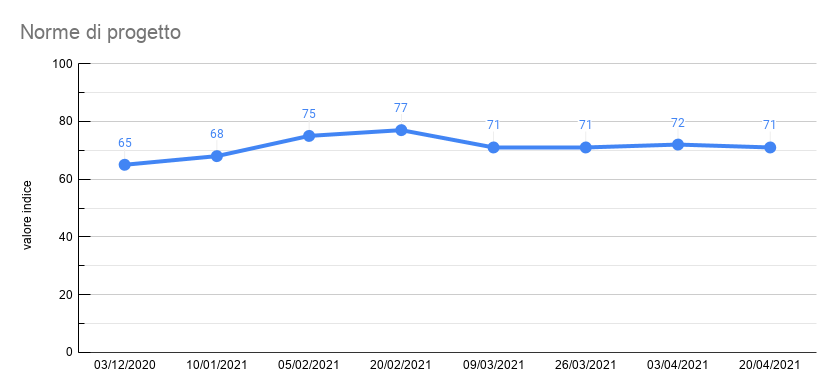
\includegraphics[width=13 cm]{source/sections/images/IdG_NdP.png}
    \caption{Indice di Gulpease - Norme di Progetto}
\end{figure}
\begin{figure}[H]
    \centering
    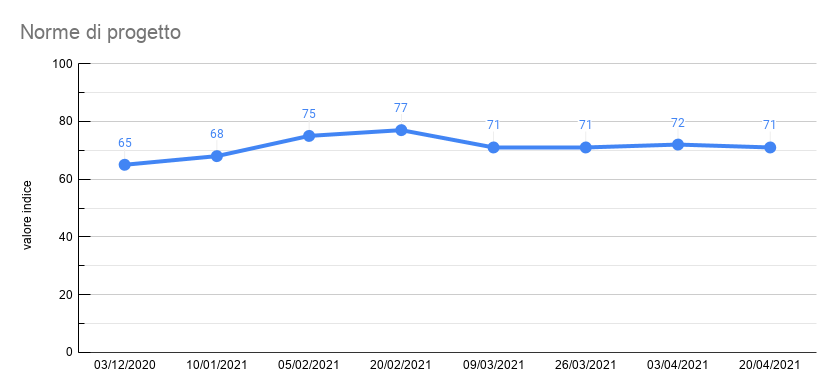
\includegraphics[width=13 cm]{source/sections/images/IdG_NdP.png}
    \caption{Indice di Gulpease - Norme di Progetto}
\end{figure}
\begin{figure}[H]
    \centering
    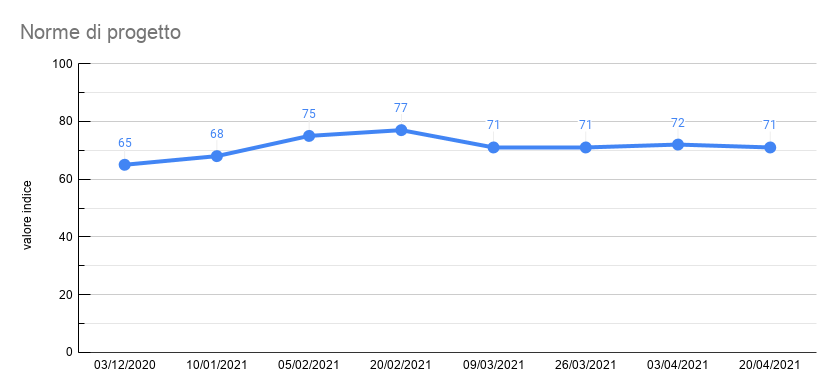
\includegraphics[width=13 cm]{source/sections/images/IdG_NdP.png}
    \caption{Indice di Gulpease - Norme di Progetto}
\end{figure}

\subsection{Errori ortografici}

Per quanto riguarda gli errori ortografici, oltre alla revisione fatta dai membri del gruppo, si è utilizzato anche lo spellchecker di Overleaf.
\newpage

\subsection{Metriche di pianificazione}
Le metriche di pianificazione che mostrano il rispettaer dei costi e dei tempi sono stati calcolati in questa versione del documento in 4 gruppi denotati dalle seguenti sigle:
\begin{itemize}
    \item \textbf{An}: Periodo di analisi, ovvero dal 26-11-2020 al 10-01-2021
    \item \textbf{CC}: periodo di consolidamento dei requisiti, ovvero dal 12-01-2021 al 18-01-2021
    \item \textbf{PA}: Progettazione architetturale, ovvero dal 19-01-2021 al 01-03-2021, che rappresenta la data progettata per la consegna
    \item \textbf{PAS}: Progettazione architetturale con consegna "a sportell0", ovvero dal 02-03-2021 al 09-03-2021, che rappresenta la data spostata con consegna il 10 marzo
\end{itemize}
In questo modo è più facile visualizzare l'andamento della pianificazione del progetto

\subsubsection{Earned value - EV}

\begin{longtabu} to \textwidth {| X[0.1,c m] | X[0.1,c m] |}
    \hline
    \rowcolor{header}
    \textbf{Fase} &
    \textbf{Valore effettivo} \\
    \hline
    An & -  \\ 
    \hline
    CR & 734 \\
    \hline
    PA & 2588 \\
    \hline
    PAS & 1035 \\
    \hline 
    \end{longtabu}

    \begin{figure}[H]
        \centering
        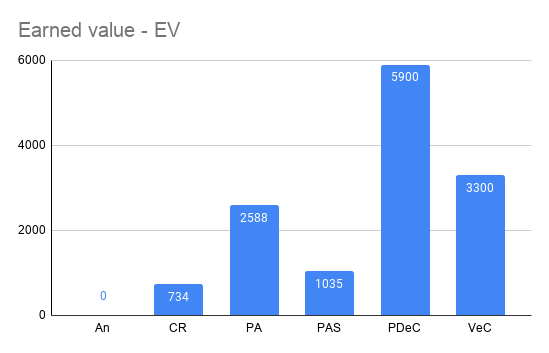
\includegraphics[width=10 cm]{source/sections/images/Earned_value.png}
        \caption{Grafico dei valori dell'Earned value}
    \end{figure}

    \newpage
\subsubsection{Planned value - PV}

\begin{longtabu} to \textwidth {| X[0.1,c m] | X[0.1,c m] | }
    \hline
    \rowcolor{header}
    \textbf{Fase} &
    \textbf{Valore effettivo} \\
    \hline
    RR & - \\
    \hline
    CR & 734 \\
    \hline
    PA & 3624 \\
    \hline
    PAS & 1035 \\
    \hline 
    \end{longtabu}

    \begin{figure}[H]
        \centering
        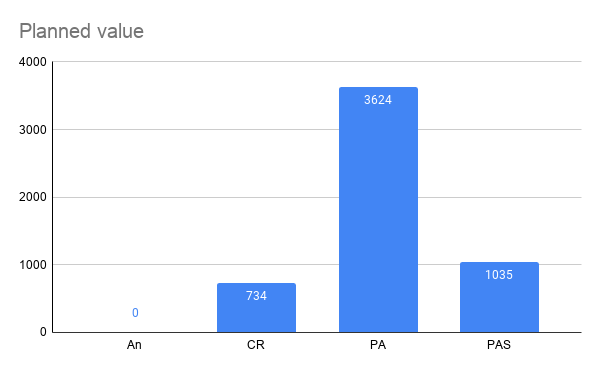
\includegraphics[width=10 cm]{source/sections/images/planned_value.png}
        \caption{Grafico dei valori del Planned value}
    \end{figure}

\subsubsection{Actual cost - AC}

\begin{longtabu} to \textwidth {| X[0.1,c m] | X[0.1,c m] | X[0.1,c m] | X[0.1,c m] |}
    \hline
    \rowcolor{header}
    \textbf{Fase} &
    \textbf{Valore effettivo} & 
    \textbf{Valore sufficiente} & 
    \textbf{Valore ottimo} \\
    \hline
    An & - & - & - \\
    \hline
    CR & 650.66 & Si & Si \\ 
    \hline    
    PA & 3439,23 & No & No \\
    \hline 
    PAS & 966 & Si & Si \\
    \hline
    \end{longtabu}

    \begin{figure}[H]
        \centering
        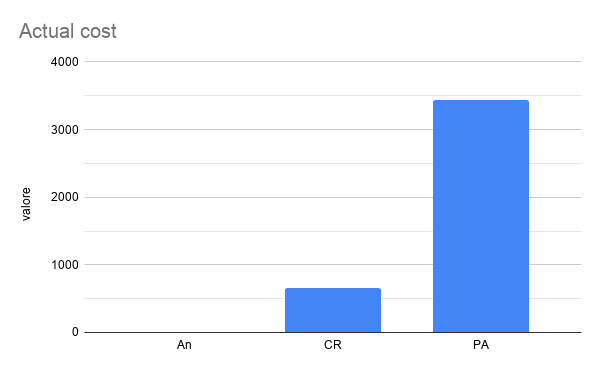
\includegraphics[width=10 cm]{source/sections/images/actual_cost.png}
        \caption{Grafico dei valori dell'Actual cost}
    \end{figure}

\subsubsection{Schedule variance - SV}

\begin{longtabu} to \textwidth {| X[0.1,c m] | X[0.1,c m] | X[0.1,c m] | X[0.1,c m]|}
    \hline
    \rowcolor{header}
    \textbf{Fase} &
    \textbf{Valore effettivo} & 
    \textbf{Valore sufficiente} & 
    \textbf{Valore ottimo} \\
    \hline
    An & - & - & - \\
    \hline
    CR & 0 & Si & Si \\ 
    \hline
    PA & -1035 & No & No \\
    \hline 
    PAS & 0 & Si & Si \\
    \hline
    \end{longtabu}

    \begin{figure}[H]
        \centering
        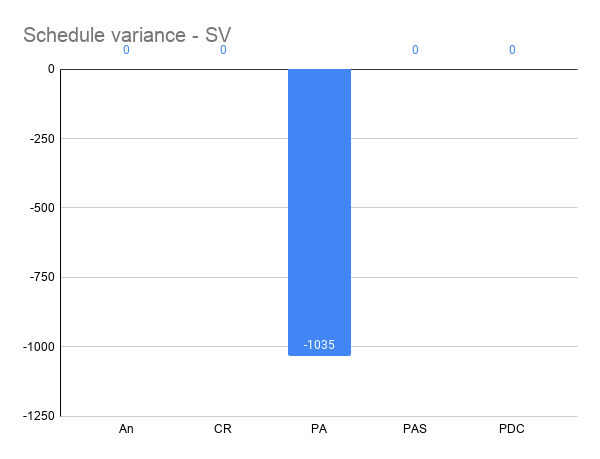
\includegraphics[width=10 cm]{source/sections/images/schedule_variance.png}
        \caption{Grafico dei valori dello Schedule variance}
    \end{figure}


\subsubsection{Cost variance - CV}
\begin{longtabu} to \textwidth {| X[0.1,c m] | X[0.1,c m] | X[0.1,c m] | X[0.1,c m]|}
    \hline
    \rowcolor{header}
    \textbf{Fase} &
    \textbf{Valore effettivo} & 
    \textbf{Valore sufficiente} & 
    \textbf{Valore ottimo} \\
    \hline
    Av & - & - & - \\ 
    \hline
    CR & 84 & Si & No \\
    \hline
    PA & -851 & No & No \\
    \hline 
    PAS & 69 & Si & No \\
    \hline
    \end{longtabu}

    \begin{figure}[H]
        \centering
        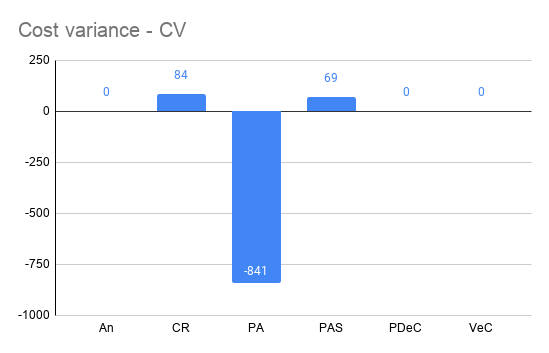
\includegraphics[width=10 cm]{source/sections/images/cost_variance.png}
        \caption{Grafico dei valori del Cost variance}
    \end{figure}
    

\subsection{Conclusioni}

\subsubsection{Analisi}
Durante il periodo di analisi tutta la documentazione da presentare in ingresso alla revisione dei requisiti è stata sottoposta ad un'analisi meticolosa della struttura del documento, della chiarezza e degli errori ortografici. La verifica di ogni documento è stata svolta da 2 componenti del gruppo per assicurare il minor numero di errori possibili.
\newline
In conclusione dai valori raggiunti dal grafico e dalla tabella soprastanti, si evince un discreto lavoro di redattori e verificatori. In particolare sono stati utili il Piano di Qualifica e le Norme di Progetto per avere un punto di riferimento, sia agli analisti nella scrittura dei documenti, sia ai verificatori per controllare con metriche e con parametri oggettivi.

\subsubsection{Consolidamento dei requisiti}
Durante questo periodo si sono svolte le attività di consolidamento in anticipazione alla Revisione dei Requisiti.
In Conclusione i valori delle metriche in questo periodo sono tutte soddifacenti ed alcune ottime, ciò indica il rispetto delle tempistiche ed una buona pianificazione da parte dei redatori del Piano di Progetto

\subsubsection{Programmazione architetturale}
Durante questo periodo si è individuata una soluzione architetturale del progetto e si è redatto il Proof of concept.
Gli scopi della programmazione architetturale non sono stati rispettati come si può vedere dalla Schedule variance con valore negativo, che indica un ritardo tamporale da parte del gruppo.
Si è così deciso di sfruttare la consegna a sportello e recuperare la progettazione, recuperando codì la perdita precedente. Si può vedere che la schedule variance del PAS è 0 che indica il rispetto delle tempistiche e l'Earned value della PAS corrisponde alle perdite del PA.
I valori del Cost variance leggermente positivi indicano una riuscita del rispetto dei costi e delle tempistiche ma senza un grande margine.
In Conclusione il gruppo è riuscito a recuperare grazie alla consegna a sportello, e non ha dovuto riconsegnare nella consegna successiva che avrebbe portato un ritardo e una perdita nei costi decisamente maggiore.